% Povinný argument: Kód předmětu
\newcommand{\subject}{MPC-ZMD}
% Povinný argument: Název předmětu
\newcommand{\subjectname}{Zpracování multimediálních dat}
% Povinný argument: Autor
\newcommand{\authorName}{<blank>}
% Povinný argument:VUT ID
\newcommand{\vutID}{<blank>}
% Nepovinný argument: Popis dokumentu
\newcommand{\docdesc}{Příloha k projektu}
% Nepovinný argument: Cílová skupina dokumentu
\newcommand{\docgroup}{}
% Nepovinný argument: URL repozitáře nebo jiný odkaz na dokument
\newcommand{\docurl}{}

% Přepsáním argumentu na 'false' vypnete balíček 'minted' pro sázení kódu.
% Pro jeho použití lokálně musíte mít v systému dostupný Python 3, python
% knihovnu 'minted' a PDFLaTeX musíte spouštět s argumentem '-shell-escape'.
% Místo něj můžete použít prostředí 'lstlisting'.
\newcommand{\docminted}{false}

% FEKT.tex
% https://github.com/VUT-FEKT-IBE/FEKT.tex
% Git hash repozitáře v době kopírování:

\documentclass[
    % Velikost základního písma je 12 bodů
    12pt,
    % Formát papíru je A4
    a4paper,
    % Oboustranný tisk
    twoside,
    % Záložky a metainformace ve výsledném PDF budou v kódování unicode
    unicode,
]{article}

%%%%%%%%%%%%%%%%%%%%
% OBECNÉ NASTAVENÍ %
%%%%%%%%%%%%%%%%%%%%

% Kódování zdrojových souborů
\usepackage[utf8]{inputenc}
% Kódování výstupního souboru
\usepackage[T1]{fontenc}
% Podpora češtiny
\usepackage[czech]{babel}

% Geometrie stránky
\usepackage[
    % Horní a dolní okraj
    tmargin=25mm,
    bmargin=25mm,
    % Vnitřní a vnější okraj
    lmargin=30mm,
    rmargin=20mm,
    % Velikost zápatí
    footskip=17mm,
    % Vypnutí záhlaví
    nohead,
]{geometry}

% Zajištění kopírovatelnosti a prohledávanosti vytvořených PDF
\usepackage{cmap}
% Podmínky (pro použití v titulní straně)
\usepackage{ifthen}

%%%%%%%%%%%%%%%
% FORMÁTOVÁNÍ %
%%%%%%%%%%%%%%%

% Nastavení stylu nadpisů
\usepackage{sectsty}
% Formátování obsahů
\usepackage{tocloft}
\setcounter{tocdepth}{1}
% Odstranění mezer mezi řádky v seznamech
\usepackage{enumitem}
\setlist{nosep}
\setitemize{leftmargin=1em}
\setenumerate{leftmargin=1.5em}
\renewcommand{\labelitemi}{--}
\renewcommand{\labelitemii}{$\circ$}
\renewcommand{\labelitemiii}{$\cdot$}
\renewcommand{\labelitemiv}{--}
% Sázení správných uvozovek pomocí '\enquote{}'
\usepackage{csquotes}
% Vynucení umístění poznámek pod čarou vespod stránky
\usepackage[bottom]{footmisc}
% Automatické zarovnání textu k předcházení vdov a parchantů
\usepackage[defaultlines=3,all=true]{nowidow}
% Zalomení části textu pokud není na současné stránce dost místa
\usepackage{needspace}

% Nastavení řádkování
\usepackage{setspace}
\onehalfspacing
% Změna odsazení odstavců
\setlength{\parskip}{1em}
\setlength{\parindent}{0em}

% Bezpatkové sázení nadpisů
\allsectionsfont{\sffamily}
% Změna formátování nadpisu a podnadpisů v Obsahu
\renewcommand{\cfttoctitlefont}{\Large\bfseries\sffamily}
\renewcommand{\cftsubsecdotsep}{\cftdotsep}

% Použití moderní/aktualizované sady písem
\usepackage{lmodern}

%%%%%%%%%%%
% NADPISY %
%%%%%%%%%%%

\usepackage{titlesec}

\titlespacing*{\section}{0pt}{10pt}{-0.2\baselineskip}
\titlespacing*{\subsection}{0pt}{0.2\baselineskip}{-0.2\baselineskip}
\titlespacing*{\subsubsection}{0pt}{0.2\baselineskip}{-0.2\baselineskip}
\titlespacing*{\paragraph}{0pt}{0pt}{1em}

%%%%%%%%%%
% ODKAZY %
%%%%%%%%%%

% Tvorba hypertextových odkazů
\usepackage[
    breaklinks=true,
    hypertexnames=false,
]{hyperref}
% Nastavení barvení odkazů
\hypersetup{
    colorlinks,
    citecolor=black,
    filecolor=black,
    linkcolor=black,
    urlcolor=blue
}

%%%%%%%%%%%%%%%%%%%%%%%%%%%
% OBRÁZKY, GRAFY, TABULKY %
%%%%%%%%%%%%%%%%%%%%%%%%%%%

% Vkládání obrázků
\usepackage{graphicx}
\usepackage{subcaption}
% Nastavení popisů obrázků, výpisů a tabulek
\usepackage{caption}
\captionsetup{justification=centering}
% Grafy a vektorové obrázky
\usepackage{tikz}
\usetikzlibrary{shapes,arrows}
% Složitější tabulky
\usepackage{tabularx}
\usepackage{multicol}

% Sázení osamocených float prostředí v horní části stránky
\makeatletter
\setlength{\@fptop}{0pt plus 10pt minus 0pt}
\makeatother

% Vynucení vypsání floating prostředí pomocí \FloatBarrier
\usepackage{placeins}

%%%%%%%%%%%%%%
% MATEMATIKA %
%%%%%%%%%%%%%%

% Sázení matematiky a matematických symbolů ('\mathbb{}')
\usepackage{amsmath}
\usepackage{amssymb}
% Sázení fyzikálních veličin
\usepackage{siunitx}

%%%%%%%%%%%%%%%%%
% ZDROJOVÉ KÓDY %
%%%%%%%%%%%%%%%%%

% Sazba zdrojových kódů
\usepackage[formats]{listings}
% Přepnutí prostředí 'code' do režimu výpisu kódu
\newenvironment{code}{\captionsetup{type=listing}}{}

\lstset{
    basicstyle=\small\ttfamily,
    numbers=left,
    numberstyle=\tiny,
    tabsize=4,
    columns=fixed,
    showstringspaces=false,
    showtabs=false,
    keepspaces,
}

% Balíček 'minted' budeme používat pouze pokud je jeho hodnota nastavena na 'true'
\providecommand{\docminted}{false}
\ifthenelse{\equal{\docminted}{true}}
{
    % Sazba zdrojových kódů
    \usepackage[newfloat]{minted}
    % Nastavení barev 'minted' kódů
    \usemintedstyle{pastie}
}
{
    % \docminted není 'true', nic neprovádíme
    % Pokud je v dokumentu 'minted' prostředí, dokument se nepodaří přeložit.
}

%%%%%%%%%%%
% TITULKA %
%%%%%%%%%%%

\IfFileExists{./.repo.tex}{
    % Soubor '.repo.tex' může (re)definovat povinné a nepovinné argumenty
    % souboru 'main.tex'. To lze využít v případech kdy v jednom repozitáři
    % existuje více dokumentů najednou (např. státnicové otázky).
    \input{.repo}
}{}

% Pokud byly nepovinné argumenty zakomentovány nebo vymazány, přidáme prázdné
% definice příkazů, aby bylo dokument možné správně přeložit.
\providecommand{\docdesc}{}
\providecommand{\docgroup}{}
\providecommand{\docurl}{}

\newcommand{\titulka}{
    \vspace*{2em}
    \begin{center}
        {\Huge \bfseries \subject}

        \vspace*{1em}

        {\Huge \bfseries \subjectname}

        \vspace*{2em}

        {\Large \docdesc}

        \vspace*{1em}

        \docgroup

        \url{\docurl}
    \end{center}

    \vfill

    \begin{tabular}{ll}
        Autor: & \authorName \\
        ID:    & \vutID      \\
    \end{tabular}
    \hfill
    \today

    \thispagestyle{empty}
    \newpage
}

\usepackage{mdframed}

\begin{document}

\titulka{}

\setcounter{page}{1}

\section[aplikace]{Aplikace}

\begin{figure}[h]
    \begin{center}
        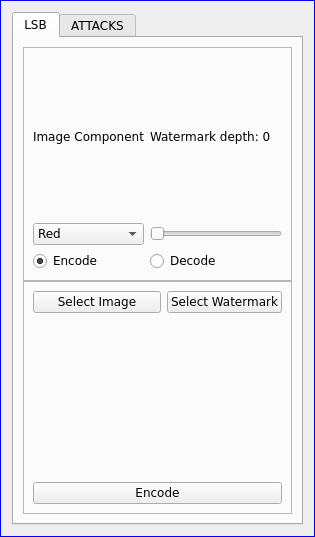
\includegraphics[scale=0.5]{images/app.jpg}
        \caption{Aplikace po spuštění}
    \end{center}
\end{figure}

Po spuštění aplikace je možné vložit/extrahovat LSB vodoznak do/z obrázku, nebo zkusit nějaký útok na již vodoznačený obrázek.

\section[lsb]{LSB Vodoznačení}

Pro vytvoření vodoznaku je třeba vybrat jakou složku obrazu využít na vodoznak a do jaké bitové hloubky bude vodoznak zasazen. Dále je třeba vybrat obrázek, který bude vodoznačen a samotný vodoznak. Pokud je vodoznak menší, než původní obrázek bude zduplikován tak, aby vyplnil celý rozsah.

\begin{figure}[h!]
    \begin{center}
        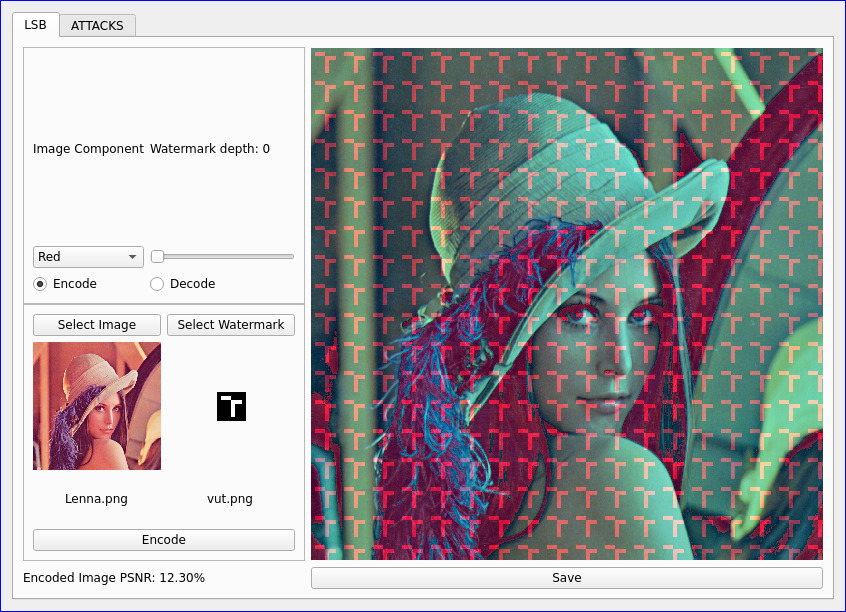
\includegraphics[scale=0.4]{images/encoding.jpg}
        \caption{Vytvoření LSB vodoznaku}
    \end{center}
\end{figure}

\begin{figure*}[h!]
    \begin{center}
        \begin{subfigure}[t]{0.5\textwidth}
            \centering
            
\includegraphics[height=8cm]{images/lsb_0.jpg}
            \caption{LSB v minimální hloubce}
        \end{subfigure}%
        ~
        \begin{subfigure}[t]{0.5\textwidth}
            \centering
            
\includegraphics[height=8cm]{images/lsb_7.jpg}
            \caption{LSB v maximální hloubce}
        \end{subfigure}
        \caption{Rozdíly v hloubkách u LSB}
    \end{center}
\end{figure*}


\clearpage


Pro extrakci vodoznaku stačí pouze vybrat obrázek, složku a hloubku.

\begin{figure}[h!]
    \begin{center}
        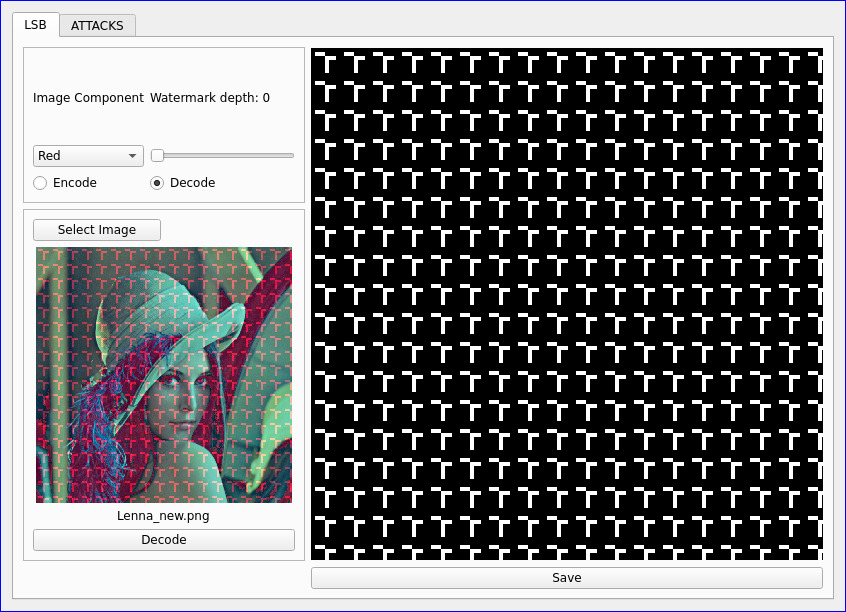
\includegraphics[scale=0.4]{images/decoding.jpg}
        \caption{Extrakce LSB vodoznaku}
    \end{center}
\end{figure}

\newpage
\section[utoky]{Útoky}
V aplikaci jsou implementovány 4 typy útoků:
\begin{itemize}
    \item JPEG Komprese
    \item Rotace a následné vrácení zpět
    \item Zmenšení velikosti
    \item Zrcadlení obrázku
\end{itemize}

\begin{figure}[h!]
    \begin{center}
        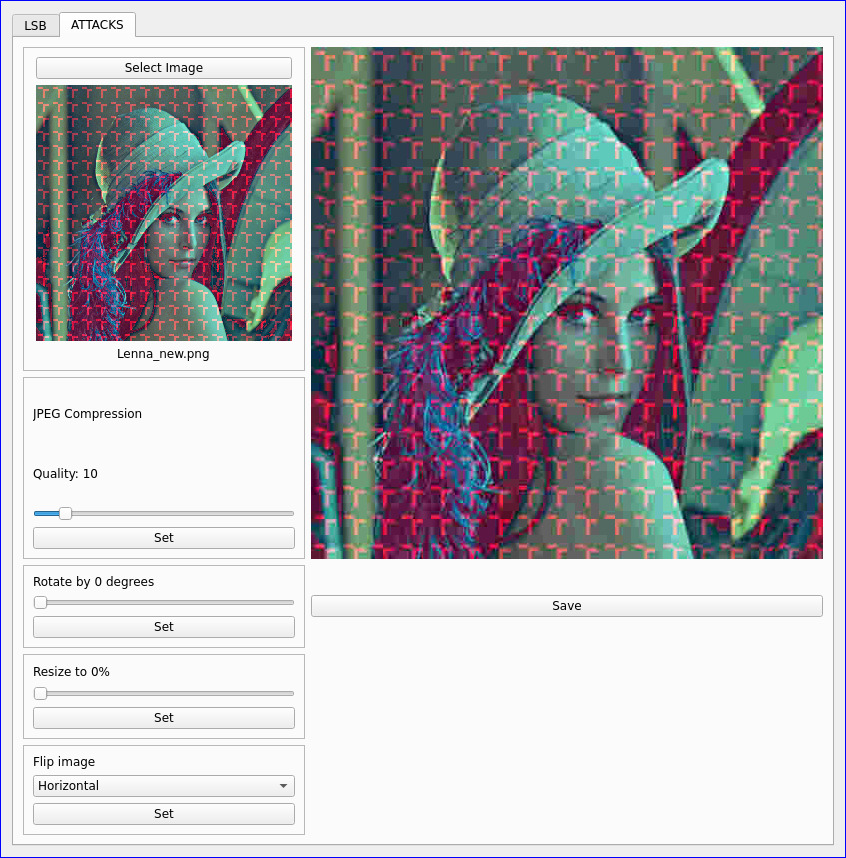
\includegraphics[scale=0.4]{images/attacks.jpg}
        \caption{Útoky na vodoznak}
    \end{center}
\end{figure}

\subsection[jpeg]{JPEG Komprese obrázku}
Komprese je velmi účinná proti vodoznaku ve velké hloubce. I velmi malá komprese dokáže vodoznak úplně zničit.

\begin{figure*}[h!]
    \begin{center}
        \begin{subfigure}[t]{0.5\textwidth}
            \centering
            
\includegraphics[height=8cm]{images/lsb_7_95_qual.jpg}
            \caption{LSB v maximální hloubce po JPEG kompresi s 95\% kvalitou}
        \end{subfigure}%
        ~
        \begin{subfigure}[t]{0.5\textwidth}
            \centering
            
\includegraphics[height=8cm]{images/lsb_7_95_qual_extracted.jpg}
            \caption{Extrahovaný obrázek}
        \end{subfigure}
        \caption{Vliv komprese na maximální hloubku vodoznaku}
    \end{center}
\end{figure*}

\begin{figure*}[h!]
    \begin{center}
        \begin{subfigure}[t]{0.5\textwidth}
            \centering
            
\includegraphics[height=8cm]{images/lsb_0_35_qual.jpg}
            \caption{LSB v minimální hloubce po JPEG kompresi s 35\% kvalitou}
        \end{subfigure}%
        ~
        \begin{subfigure}[t]{0.5\textwidth}
            \centering
            
\includegraphics[height=8cm]{images/lsb_0_35_qual_extracted.jpg}
            \caption{Extrahovaný obrázek}
        \end{subfigure}
        \caption{Vliv komprese na minimální hloubku vodoznaku}
    \end{center}
\end{figure*}

\clearpage

\subsection[rotace]{Rotace obrázku}
Rotace je implementována tak, že obrázek se při první rotaci zvětší tak, aby mu nebyly oříznuty rohy a po rotaci zpět je oříznut zpět na původní velikost. Z tohoto důvodu nemá rotace velký vliv na extrahovaný vodoznak, pouze do něj vnese drobný šum.

\begin{figure}[h!]
    \begin{center}
        
\includegraphics[scale=0.4]{images/rotation_30deg.jpg}
        \caption{Obrázek po první rotaci}
    \end{center}
\end{figure}

\begin{figure*}[h!]
    \begin{center}
        \begin{subfigure}[t]{0.5\textwidth}
            \centering
            
\includegraphics[height=8cm]{images/rotation_30deg_fin.jpg}
            \caption{Obrázek po rotaci o 30\textdegree{}, zpět a po oříznutí okrajů}
        \end{subfigure}%
        ~
        \begin{subfigure}[t]{0.5\textwidth}
            \centering
            
\includegraphics[height=8cm]{images/rotation_30deg_extracted.jpg}
            \caption{Extrahovaný obrázek}
        \end{subfigure}
        \caption{Vliv rotace na vodoznak}
    \end{center}
\end{figure*}

\clearpage
\subsection[zmenseni]{Zmenšení velikosti obrázku}
Podobně jako JPEG komprese, i změna velikosti obrázku výrazně ovlivňuje vodoznak.

\begin{figure*}[h!]
    \begin{center}
        \begin{subfigure}[t]{0.5\textwidth}
            \centering
            
\includegraphics[height=8cm]{images/resize_7_75percent.jpg}
            \caption{Obrázek po zmenšení na 75\%}
        \end{subfigure}%
        ~
        \begin{subfigure}[t]{0.5\textwidth}
            \centering
            
\includegraphics[height=8cm]{images/resize_7_75percent_extracted.jpg}
            \caption{Extrahovaný obrázek}
        \end{subfigure}
        \caption{Vliv zmenšení na vodoznak v maximální hloubce}
    \end{center}
\end{figure*}

\begin{figure*}[h!]
    \begin{center}
        \begin{subfigure}[t]{0.5\textwidth}
            \centering
            
\includegraphics[height=8cm]{images/resize_0_75percent.jpg}
            \caption{Obrázek po zmenšení na 75\%}
        \end{subfigure}%
        ~
        \begin{subfigure}[t]{0.5\textwidth}
            \centering
            
\includegraphics[height=8cm]{images/resize_0_75percent_extracted.jpg}
            \caption{Extrahovaný obrázek}
        \end{subfigure}
        \caption{Vliv zmenšení na vodoznak v minimální hloubce}
    \end{center}
\end{figure*}

\clearpage
\subsection[zrcadleni]{Zrcadlení obrázku}
Zrcadlení obrázku nemá žádný vliv na výsledný vodoznak, ten je pouze zrcadlený úplně stejně jako samotný obrázek.

\begin{figure*}[h!]
    \begin{center}
        \begin{subfigure}[t]{0.5\textwidth}
            \centering
            
\includegraphics[height=8cm]{images/flip_horizontal.jpg}
            \caption{Obrázek po horizontálním zrcadlení}
        \end{subfigure}%
        ~
        \begin{subfigure}[t]{0.5\textwidth}
            \centering
            
\includegraphics[height=8cm]{images/flip_horizontal_extracted.jpg}
            \caption{Extrahovaný obrázek}
        \end{subfigure}
        \caption{Vliv horizontálního zrcadlení na vodoznak v maximální hloubce}
    \end{center}
\end{figure*}

\begin{figure*}[h!]
    \begin{center}
        \begin{subfigure}[t]{0.5\textwidth}
            \centering
            
\includegraphics[height=8cm]{images/flip_vertical.jpg}
            \caption{Obrázek po vertikálním zrcadlení}
        \end{subfigure}%
        ~
        \begin{subfigure}[t]{0.5\textwidth}
            \centering
            
\includegraphics[height=8cm]{images/flip_vertical_extracted.jpg}
            \caption{Extrahovaný obrázek}
        \end{subfigure}
        \caption{Vliv vertikálního zrcadlení na vodoznak v minimální hloubce}
    \end{center}
\end{figure*}

\end{document}
